\chapter{ Performance Benchmarking }
\label{sec:bench}

To investigate the feasibility of WebAssembly (WASM) as a universal distributable for embedded audio applications, I have compiled four representative audio processing routines to WASM with a consistent binary interface using Emscripten\cite{emscripten} and measured execution time of each across three WASM runtimes on a resource contained target. For a baseline reference, I compiled and benchmarked each of the four routines as native ARM code as well via \lstinline{gcc-arm-none-eabi} invoked with an optimization level of \lstinline{-Ofast}.

% \begin{itemize}
%   \item A FAUST spring reverb exported to C++
%   \item A Gen\textasciitilde{} phaser exported to C++
%   \item A virtual analog model of a Klon Centaur overdrive circuit
%   \item A lightweight implementation of Neural Amp Modeler
% \end{itemize}

\section{ Algorithms }

In order to contextualize this research relative to real-world applications, I sourced a set of DSP algorithms that span major paradigms in both contemporary audio effects design and development workflows.

% \bigskip

% \noindent \textbf{ FAUST Reverb }
\subsection{ FAUST Reverb}

The FAUST domain-specific programming language (DSL) is popular among audio developers for its capability to generate code for many different targets to be compiled separately, as well as its high-level semantics for describing audio DSP. The maintainers of FAUST supply many example programs, including a reverb algorithm I have used here. The algorithm uses physical modeling techniques to emulate a spring reverb effect.

% \bigskip

\subsection{ Gen\textasciitilde \space Phaser }

Gen\textasciitilde \space is another popular domain-specific programming language (DSL) for audio. A major difference from FAUST is that Gen\textasciitilde \space is a \textit{visual} programming language, providing a user interface that is often less challenging for beginners. Like many other audio DSLs, Gen\textasciitilde \space provides the ability to export code to target different platforms. For the purposes of benchmarking, I used Gen\textasciitilde \space to construct an elementary phaser effect with four cascaded state variable filters (from the GO library\cite{BD0831917X}) and a low-frequency oscillator.

\subsection{ Klon Centaur }

The Klon Centaur is a highly acclaimed guitar overdrive pedal designed in the 1990s, whose circuitry has been copied in analog and digital forms many times over\cite{chowdhury2020comparison}. Prominent audio DSP programmer and scholar Jatin Chowdhury maintains an open-source C++ implementation using wave digital filters, a popular technique in audio DSP for white-box modeling of analog circuits.

\subsection{ Neural Amp Modeler }

Neural Amp Modeler (NAM)\cite{neuralampmodeler} is a free and open-source standard for black-box modeling of audio equipment using neural networks. It has become highly popular in both hobbyist communities and industry, but implementations vary widely across platforms. For this benchmark I have used a C++ implementation of a NAM inference engine authored by Keith Bloemer\cite{guitarml_mercury}, written specifically for use on an embedded platform.

% https://github.com/GuitarML/FunBox/blob/main/software/Mars/mars.cpp

\section{ Runtimes }

To compare deployment strategies for WASM-based audio DSP on an embedded target, three distinct execution pipelines were selected for evaluation. They represent three fundamentally different approaches to executing WASM modules: ahead-of-time (AOT) compilation paired with an embedded-focused runtime, static translation to C followed by conventional compilation, and pure interpretation.

\subsection{ Wasm Micro Runtime (WAMR) }

The WebAssembly Micro Runtime (WAMR), maintained by the Bytecode Alliance\cite{bytecode_alliance}, is a lightweight WASM runtime explicitly designed for embedded systems. It supports multiple execution modes, including interpretation and AOT translation. For this study, WAMR was used in AOT mode, in which WASM bytecode is compiled offline into target-specific native machine code. The resulting artifact is managed by the WAMR runtime, which provides memory management, stack handling, and host function bindings.

\subsection{ wasm2c }

\lstinline{wasm2c} is a tool provided in the WebAssembly Binary Toolkit (WABT)\cite{wabt-repo} that translates WASM modules into C source code. Unlike WAMR, \lstinline{wasm2c} is not a "runtime" in the traditional sense; it is a static translation step. I have leveraged a thin "runtime" implemented by wasm3labs\cite{embedded-wasm-apps_repo} to manage exported modules.


\subsection{ wasmi }

\lstinline{wasmi}\cite{wasmi} is a pure WebAssembly interpreter written in Rust. It executes WASM bytecode directly using a stack-based virtual machine, without just-in-time (JIT) or AOT compilation. Wasmi was selected to represent a baseline interpreter-only deployment strategy, providing contrast to AOT-based approaches by illustrating the performance cost of direct bytecode interpretation.

\section { Embedded Target }

I have chosen the Electrosmith Daisy Seed as a representative platform for benchmarking embedded processing. Daisy is a widely popular embedded platform, similar to the Arduino\cite{arduino} ecosystem but with a focus on audio. The STM32 processor at its core is widely used across research and industry for embedded audio systems\cite{emilyharpist}\cite{diamond2025memorylane}\cite{jongsataporn2025embedded}.

\section { Benchmarking Code }

To benchmark execution time, the STM32H7's TIM2 hardware counter is leveraged to measure elapsed time in both raw tick counts and microseconds. Timer \lstinline{start()} and \lstinline{stop()} calls bookend calls to the WASM runtimes to process 128-sample blocks of audio data. For each algorithm and runtime combination, the elapsed time is averaged over 100 iterations. A 400MHz clock rate is used. The source code for benchmarks on WAMR, \lstinline{wasm2c}, and \lstinline{wasmi} are available at \cite{wamrRepo}, \cite{wasm2cRepo}, and \cite{wasmiRepo}, respectively, with dedicated Git branches for benchmarking each algorithm. Native benchmarking is included in \lstinline{wasm2c-demo}. Quantitative results are presented in \autoref{tab:throughput_raw}, \autoref{tab:relative_performance}, and \autoref{fig:relative_performance}.

\vspace{12pt}

\begin{table}[ht]
\caption{\itshape Raw sample throughput (samples/sec) across runtimes. \\
Cells shaded green represent algorithm/runtime combinations with throughput greater than 48kHz, indicating real-time performance}
\centering
\resizebox{\columnwidth}{!}{
\begin{tabular}{|l|c|c|c|c|}
  \hline
  Algorithm & Native & WAMR AOT & Wasm2c & Wasmi \\
  \hline
  FAUST Reverb
    & \cellcolor{green!20} 76,141
    & \cellcolor{green!20} 67,288
    & \cellcolor{green!20} 65,222
    & \cellcolor{red!20} 6,259 \\
  Gen\textasciitilde{} Phaser
    & \cellcolor{green!20} 345,862
    & \cellcolor{green!20} 189,599
    & \cellcolor{green!20} 215,242
    & \cellcolor{red!20} 974 \\
  Klon Centaur
    & \cellcolor{green!20} 142,487
    & \cellcolor{red!20} 32,880
    & \cellcolor{red!20} 38,030
    & \cellcolor{red!20} --* \\
  Neural Amp Modeler
    & \cellcolor{green!20} 76,759
    & \cellcolor{red!20} 5,565
    & \cellcolor{red!20} 22,237
    & \cellcolor{red!20} --* \\
  \hline
\end{tabular}
}
\label{tab:throughput_raw}
\end{table}


\begin{table}[ht]
\caption{\itshape Relative performance comparison of different algorithms across runtimes. }
\centering
\resizebox{\columnwidth}{!}{
\begin{tabular}{|l|c|c|c|c|}
  \hline
  Algorithm & Native & WAMR AOT & Wasm2c & Wasmi \\
  \hline
  FAUST Reverb
    & \cellcolor{green!20} 1.0x
    & \cellcolor{green!20} 0.8837x
    & \cellcolor{green!20} 0.8566x
    & \cellcolor{red!20} 0.0822x \\
  Gen\textasciitilde{} Phaser
    & \cellcolor{green!20} 1.0x
    & \cellcolor{green!20} 0.5482x
    & \cellcolor{green!20} 0.6223x
    & \cellcolor{red!20} 0.0028x \\
  Klon Centaur
    & \cellcolor{green!20} 1.0x
    & \cellcolor{red!20} 0.2308x
    & \cellcolor{red!20} 0.2669x
    & \cellcolor{red!20} --* \\
  Neural Amp Modeler
    & \cellcolor{green!20} 1.0x
    & \cellcolor{red!20} 0.0725x
    & \cellcolor{red!20} 0.2897x
    & \cellcolor{red!20} --* \\
  \hline
\end{tabular}
}
\label{tab:relative_performance}
\end{table}

{\footnotesize *Algorithm/runtime combination did not achieve stable performance}

\FloatBarrier  % may be needed

\begin{figure}[htbt]
\centering
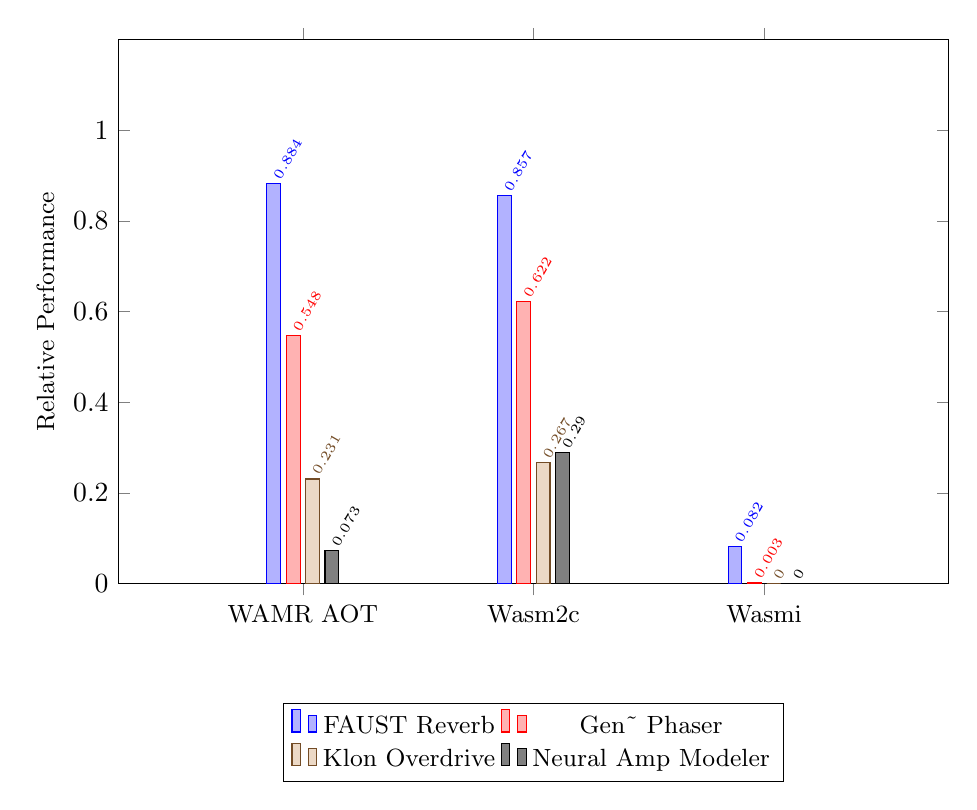
\begin{tikzpicture}
\begin{axis}[
    ybar,
    width=\columnwidth,
    height=0.7\columnwidth,
    bar width=12pt,
    enlarge x limits=0.4,
    bar width=5pt,
    ymin=0,
    ymax=1.2,
    ylabel={Relative Performance},
    symbolic x coords={WAMR AOT, Wasm2c, Wasmi},
    xtick=data,
    % ytick distance={1}
    ytick={0, 0.2, 0.4, 0.6, 0.8, 1.0},
    xticklabel style={font=\small},
    ylabel style={font=\small},
    legend style={
        at={(0.5,-0.22)},
        anchor=north,
        legend columns=2,
        font=\small
    },
    nodes near coords,
    nodes near coords style={
        font=\tiny,         % Smaller font for dense data
        rotate=60,          % Rotate to prevent overlap
        anchor=west,        % Align to the top of the bar
        inner sep=2pt,      % Padding from the bar top
        /pgf/number format/fixed,
        /pgf/number format/precision=3
    },
]

\addplot coordinates {(WAMR AOT,0.8837) (Wasm2c,0.8566) (Wasmi,0.0822)};
\addplot coordinates {(WAMR AOT,0.5482) (Wasm2c,0.6223) (Wasmi,0.0028)};
\addplot coordinates {(WAMR AOT,0.2308) (Wasm2c,0.2669) (Wasmi,0.0)};
\addplot coordinates {(WAMR AOT,0.0725) (Wasm2c,0.2897) (Wasmi,0.0)};

\legend{
FAUST Reverb,
Gen\textasciitilde{} Phaser,
Klon Overdrive,
Neural Amp Modeler
}

\end{axis}
\end{tikzpicture}
\caption{\it Performance comparison relative to native (1.0x).}
\label{fig:relative_performance}
\end{figure}

\vspace{12pt}
